\documentclass[./Thesis.tex]{subfiles}
\begin{document}

\chapter{Termination}
\label{chap:termination}

\epigraph{
  What can be asserted without evidence can also be dismissed without evidence.
}{Christopher Hitchens \cite{hitchens-quote}}

\begin{code}[hide]
  module Termination where
  open import Relation.Nullary.Decidable using (False)
  open import Relation.Nullary.Negation using (contradiction)
  open import Data.Empty using (⊥)
  open import AKS.Nat using (ℕ; zero; suc; _*_; _<_; _≤_; lte; _≟_)
  open import AKS.Nat using (+-comm; suc-injective-≡)
  open import AKS.Binary using (𝔹⁺)
  open 𝔹⁺
  open import AKS.Nat.Divisibility using (_div_; Euclidean; Euclidean✓)
  open Euclidean using () renaming (q to quotient)
  open import Relation.Binary.PropositionalEquality
    using (_≡_; _≢_; module ≡-Reasoning)
    renaming (refl to ≡-refl; sym to ≡-sym; cong to ≡-cong; cong₂ to ≡-cong₂)
  open ≡-Reasoning
  open import Data.Unit using (tt)
  open import Polynomial.Simple.AlmostCommutativeRing.Instances using (module Nat)
  open import Polynomial.Simple.Reflection using (solve)
  open Nat.Reflection using (∀⟨_⟩)
  open import Data.List using ([]; _∷_)
  open import Function using (_$_)
\end{code}
\section{A Correctness Interlude}
\label{sec:a-correctness-interlude}
The previous chapter omitted a critical flaw in it's analysis. The code below is
rejected by the \Agda{} compiler. The compiler's \textit{termination checker} \cite{agda}
fails as \Agda{} can not infer that the result of non zero integer division by
two always returns an integer strictly smaller than the input. The termination
checker ensures than every function is total or in other
words the termination checker disallows infinite loops. This termination proof
is obvious but termination proofs can quickly become complex. Famously checking
termination, commonly called the halting problem is undecidable. 
\begin{code}[hide]
  module Bad₁ where
    {-# TERMINATING #-}
\end{code}
\begin{code}
    ⟦_⇑⟧⁺ : ∀ (n : ℕ) {≢0 : False (n ≟ 0)} → 𝔹⁺
    ⟦ suc n ⇑⟧⁺ with suc n div 2
    ... | Euclidean✓ (suc q) 0 _ _ = ⟦ suc q ⇑⟧⁺ 0ᵇ
    ... | Euclidean✓ zero    1 _ _ = 𝕓1ᵇ
    ... | Euclidean✓ (suc q) 1 _ _ = ⟦ suc q ⇑⟧⁺ 1ᵇ
\end{code}
This checker is a keystone of the correctness of the logic of \Agda{}. Consider
the following function with a similar call graph. Instead of the input
decreasing to some base case it doubles every recursive call. This function can
be used to prove falsehood, thus a logic with unconstrained recursion is
inconsistent.
\begin{code}[hide]
  module Bad₂ where
    {-# TERMINATING #-}
\end{code}
\begin{code}
    increasing : ℕ → ⊥
    increasing n with 2 * n
    ... | q = increasing q

    false : ⊥
    false = increasing 0
\end{code}
In fact the example above can be simplified in the following code. In English
this code expresses the famous fallacy of circular reasoning ``false is true
because false is true''.
\begin{code}[hide]
  module Bad₃ where
    {-# TERMINATING #-}
\end{code}
\begin{code}
    false : ⊥
    false = false
\end{code}
Thankfully none of these false expressions are accepted by the \Agda{} compiler.
This begs the question how does \Agda{} determine which recursive functions to
accept. How can it solve the halting problem? The answer is unsurprisingly it
does not solve the halting problem. Instead the compiler only accepts recursive
calls that are \textit{structurally decreasing}, a small
subset of the set of recursive functions. A recursive call is structurally
decreasing if the call occurs on a strict sub expression \cite{agda}. The
expression $\AgdaInductiveConstructor{suc} \, n$ is a strict sub expression of
$\AgdaInductiveConstructor{suc} \,
  (\AgdaInductiveConstructor{suc} \,
    (\AgdaInductiveConstructor{suc} \, n))
$
but $\AgdaInductiveConstructor{suc} \, n$ is not a strict sub expression of
$\AgdaInductiveConstructor{suc} \, n$.
Addition, our first example of recursion, is acceptable as
$n <_{sub} \AgdaInductiveConstructor{suc} \, n$.
\begin{code}[hide]
  module Add where
\end{code}
\begin{code}
    _+_ : ℕ → ℕ → ℕ
    zero + m = m
    (suc n) + m = suc (n + m)
\end{code}
\begin{code}[hide]
  open import AKS.Nat using (_+_)
\end{code}
The following inductive definition of Fibonacci
has structurally decreasing calls as
$\AgdaInductiveConstructor{suc} \, n <_{sub} \AgdaInductiveConstructor{suc} \, (\AgdaInductiveConstructor{suc} \, n)$
and
$n <_{sub} \AgdaInductiveConstructor{suc} \, (\AgdaInductiveConstructor{suc} \, n)$.
\begin{code}
  fib : ℕ → ℕ
  fib zero = 0
  fib (suc zero) = 1
  fib (suc (suc n)) = fib (suc n) + fib n
\end{code}
So far all the recursive functions described have been
\textit{primitive recursive} \cite{soare}. This is a large class but the set of
structurally decreasing functions is larger than the set of primitive
recursive functions. The Ackerrmann function is the conical example of a non
primitive recursive function. \begin{code}
  ack : ℕ → ℕ → ℕ
  ack zero m = suc m
  ack (suc n) zero = ack n (suc zero)
  ack (suc n) (suc m) = ack n (ack (suc n) m)
\end{code}
\Agda{} accepts this definition as the recursive
calls are decreasing lexicographically.
The recursive call in the second case decreases in the first argument so
the second argument increasing is acceptable
$
(n, \, \AgdaInductiveConstructor{suc} \, \AgdaInductiveConstructor{zero})
<_{sub}
(\AgdaInductiveConstructor{suc} \, n, \, \AgdaInductiveConstructor{zero})
$.
For a similar reason the outer call in the third case is acceptable
$
(n, \, \AgdaFunction{ack} \, (\AgdaInductiveConstructor{suc} \, n) \, m)
<_{sub}
(\AgdaInductiveConstructor{suc} \, n, \, \AgdaInductiveConstructor{suc} \, m)
$.
The inner call is acceptable as the second argument decreases while the first
stays constant, this is lexicographic order
$
(\AgdaInductiveConstructor{suc} \, n, \, m)
<_{sub}
(\AgdaInductiveConstructor{suc} \, n, \, \AgdaInductiveConstructor{suc} \, m)
$. \\

An astute reader may have noticed a pattern. \Agda{} accepts your recursive
definition if it can infer a structural \textit{well founded relation}
\cite{soare}.
\begin{align}
  \label{eqn:wellfounded-linear}
  0 < 1 < 2 < 3 < 4 < 5
\end{align}

\begin{figure}[h]
  \centering
  \begin{tikzpicture}
    \Tree
    [.3
      {$0 < 3$}
      [.{$1 < 3$}
        {$0 < 1$}
      ]
      [.{$2 < 3$}
        {$0 < 2$}
        [.{$1 < 2$}
          {$0 < 1$}
        ]
      ]
    ]
  \end{tikzpicture}
  \caption{A well founded tree }
  \label{fig:wellfounded-tree}
\end{figure}

\begin{code}
  data Acc {A : Set} (_<_ : A → A → Set) (bound : A) : Set where
    acc : (∀ {lower} → lower < bound → Acc _<_ lower)
        → Acc _<_ bound

  subrelation
      : ∀ {A : Set} {_<₁_ : A → A → Set} {_<₂_ : A → A → Set} {n}
      → (∀ {a b} → a <₂ b → a <₁ b)
      → Acc _<₁_ n
      → Acc _<₂_ n
  subrelation <₂⇒<₁ (acc down) =
    acc λ x<₂n → subrelation <₂⇒<₁ (down (<₂⇒<₁ x<₂n))

  data _≤ⁱ_ (n : ℕ) (m : ℕ) : Set where
    ≤-same : n ≡ m → n ≤ⁱ m
    ≤-step : ∀ {o} → suc o ≡ m → n ≤ⁱ o → n ≤ⁱ m

  _<ⁱ_ : ℕ → ℕ → Set
  n <ⁱ m = suc n ≤ⁱ m

  <ⁱ-well-founded : ∀ {n} → Acc _<ⁱ_ n
  <ⁱ-count-down : ∀ {m n} → m <ⁱ n → Acc _<ⁱ_ m

  <ⁱ-well-founded {n} = acc (λ x<ⁱn → <ⁱ-count-down x<ⁱn)
  <ⁱ-count-down {m} {suc .m} (≤-same ≡-refl) = <ⁱ-well-founded {m}
  <ⁱ-count-down {m} {suc n} (≤-step ≡-refl m≤n) = <ⁱ-count-down {m} {n} m≤n

  ≤⇒≤ⁱ : ∀ {a b} → a ≤ b → a ≤ⁱ b
  ≤⇒≤ⁱ {a} {b} (lte k a+k≡b) = loop a b k $ begin
    k + a ≡⟨ +-comm k a ⟩ a + k ≡⟨ a+k≡b ⟩ b ∎
    where
    loop : ∀ a b k → k + a ≡ b → a ≤ⁱ b
    loop a b zero 0+a≡b = ≤-same $ begin
      a ≡⟨⟩ 0 + a ≡⟨ 0+a≡b ⟩ b ∎
    loop a (suc b) (suc k) 1+k+a≡1+b = ≤-step ≡-refl $ loop a b k $ begin
      k + a ≡⟨ suc-injective-≡ 1+k+a≡1+b ⟩ b ∎

  <⇒<ⁱ : ∀ {a b} → a < b → a <ⁱ b
  <⇒<ⁱ {a} {b} a<b = ≤⇒≤ⁱ {suc a} {b} a<b

  <-well-founded : ∀ {n} → Acc _<_ n
  <-well-founded {n} = subrelation <⇒<ⁱ <ⁱ-well-founded
\end{code}

\begin{code}
  div-< : ∀ n q r {q≢0 : False (q ≟ 0)} → n ≡ r + 2 * q → q < n
\end{code}
\begin{code}[hide]
  div-< n (suc q) r ≡-refl = lte (q + r) (∀⟨ q ∷ r ∷ [] ⟩)
\end{code}
\begin{code}
  ⟦_,_⇑⟧ʰ : ∀ (n : ℕ) (acc : Acc _<_ n) {≢0 : False (n ≟ 0)} → 𝔹⁺
  ⟦ suc n , acc down ⇑⟧ʰ with suc n div 2
  ... | Euclidean✓ (suc q) 0 pf _ = ⟦ suc q , down (div-< (suc n) (suc q) 0 pf) ⇑⟧ʰ 0ᵇ
  ... | Euclidean✓ zero    1 _ _ = 𝕓1ᵇ
  ... | Euclidean✓ (suc q) 1 pf _ = ⟦ suc q , down (div-< (suc n) (suc q) 1 pf) ⇑⟧ʰ 1ᵇ

  ⟦_⇑⟧⁺ : ∀ (n : ℕ) {≢0 : False (n ≟ 0)} → 𝔹⁺
  ⟦ suc n ⇑⟧⁺ = ⟦ suc n , <-well-founded ⇑⟧ʰ
\end{code}

\end{document}
